  \section{Nodes}
  \subsection{Set up}
    \begin{enumerate}
      \item Ensure the node is plugged in and the switch is in the "ON" position.
      The red light will be illuminated on the node when there is power. If the node
      has already been activated on the hub you are done or else move to step 2.

      \item If this is the first time the node is being connected to the hub.
      You will need to activate it on the hub. To do this you will need a device
      capable of connecting to a wi-fi network, such as a smart phone. Under networks
      you should see a network called "SetUpGadget\_FPFDHI". Note that the "FPFDHI"
      can be any sequence of letters and is specific to the node. Connect to that network.
      Once connected you may get a warning that the network does not have access
      to the internet. That is normal proceed anyway.

      \item Open your browser and navigate to "192.168.4.1". This will bring up
      a wifi log in page. Here you will type in the hub information.
      \begin{center}
      
\includegraphics[scale=1]{images/ip-enter.png}
    \end{center}

      \item For the wifi name type "StratusPrint" and for the password "FusRoDah".
      These are the default wifi mane and password for the hub and can be changed later.

      \item Click save. If successful the "SetUpGadget\_FPFDHI" should disappear
      from your visible networks. This should take 1-3 mins. If the network is still
      visible please turn off and on your wifi again to confirm. If it is still there
      please start over from step 2 and make sure you correctly input the information.
      \begin{center}
      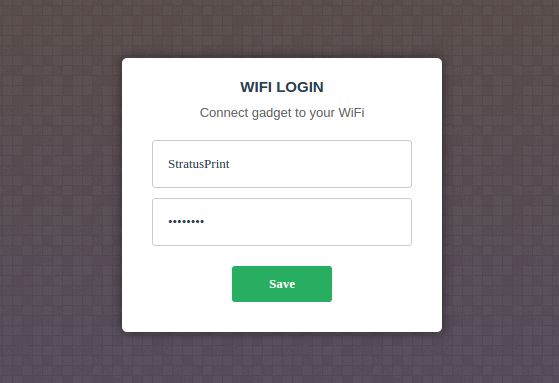
\includegraphics[scale=0.25]{images/wifi-login.png}
    \end{center}
    \end{enumerate}

  \subsection{Sensors}
  \subsubsection{Node Pinout}
  \begin{center}
        \includegraphics[scale=0.05]{images/node-pin-out.png}
  \end{center}
    \subsubsection{Job Button}
      The "Job Button" is a momentary push button that tells the hub that the bed
      is clear and it okay to start the next print. This is to provide an easy way
      for someone to clean the print bed and continue the print queue.\\

      \textbf{Operation}\\
      Once a print is complete this button will blink repeatedly until it is pressed.
      When the button is pressed it tells the hub its clear to start the next job in the
      print queue.\\

      \textbf{Wiring Diagram}\\
            \begin{center}
      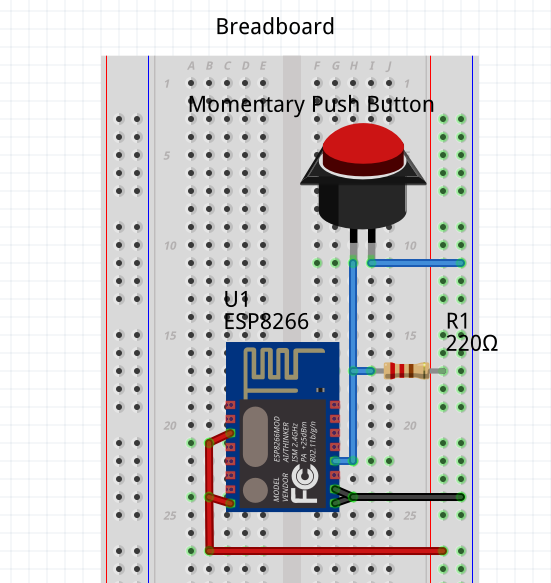
\includegraphics[scale=0.25]{images/job-cir.png}
      \end{center}
    \subsubsection{Temperature and Humidity}
      The temperature and humidity sensor will report the current room conditions. It
      can detect dangerous conditions for 3D printing and act as an early warning system
      if the conditions may lead to print.\\

      \textbf{Wiring Diagram}\\
            \begin{center}
      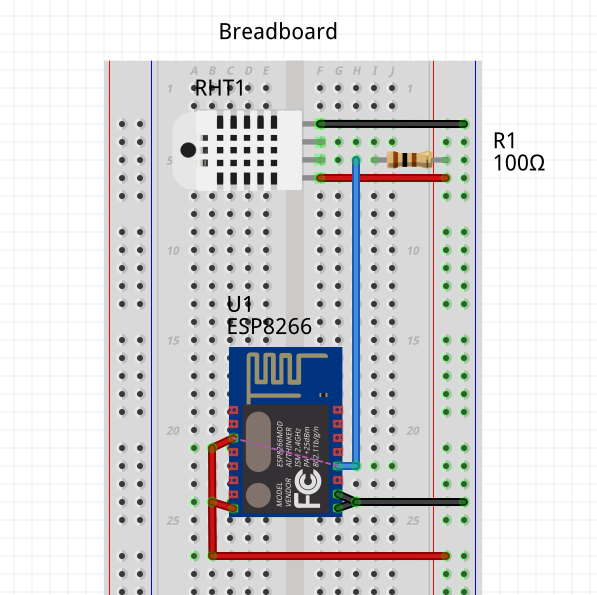
\includegraphics[scale=0.25]{images/temp-diagram.png}
\end{center}

    \subsubsection{Door Sensor}
      The door sensor is a magnetic switch mounted to the entrance of the printing lab.
      This allows for detection of an open or closed door. Which may affect printing conditions.\\

      \textbf{Wiring Diagram}\\
      \begin{center}
        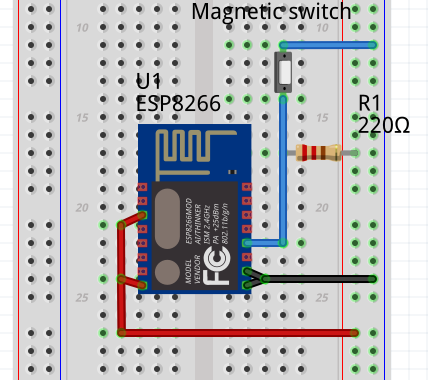
\includegraphics[scale=0.25]{images/door-cir.png}
        \end{center}
    \subsubsection{Additional Sensors}
      The nodes where set up to be universal and by that are compatible with
      many sensors because of this the nodes come with a breadboard so they can
      easily be reconfigured.\\
\newpage
  \subsection{Troubleshooting}
  \subsubsection{Reset}
  Turn the switch the the off position and unplug the node.
  \subsubsection{Node is not connecting to the hub}
  \begin{enumerate}
    \item Ensure the node has the correct wifi credentials. If the default is not
    working make sure the password hasn't been changed.
    \item If the node seems to be connected and isn't communication hard reset and re-connect.
  \end{enumerate}
  \subsubsection{Node is connected but no data is being sent from the sensors}
  Make sure the sensors are connected correctly you can reference the wiring diagrams
  in this manual.